\documentclass[a4paper, twoside]{article}

% 引入的宏包
\usepackage[UTF8]{ctex}          % 中文支持
% \usepackage{xeCJK}
\usepackage{fontspec}            % 字体设置

% 页面布局与样式
\usepackage{geometry}            % 页面布局
\usepackage{fancyhdr}            % 页眉页脚
\usepackage{setspace}            % 行间距调整
\usepackage{afterpage}           % 页面控制
\usepackage{tocloft}             % 目录样式定制
\usepackage{titlesec}            % 自定义章节标题格式
\usepackage{enumitem}            % 列表环境增强
\usepackage{booktabs}            % 表格
\usepackage{float}               % 浮动环境

% 图像与背景
\usepackage{graphicx}            % 插入图片
\usepackage{wallpaper}           % 背景设置

% 超链接与交互
\usepackage[colorlinks=true, linkcolor=black]{hyperref} % 超链接
\usepackage{nameref}             % 名称引用

% 文本格式
\usepackage{textcomp}            % 提供文本符号(如 € 等)
\usepackage{relsize}             % 改变字体相对大小
\usepackage[normalem]{ulem}      % 提供下划线、删除线等效果
\usepackage{verbatim}            % 原始文本插入

% 代码与格式化
\usepackage{listings}            % 插入代码块
\usepackage{minted}              % 代码高亮
\usepackage{color, xcolor}       % 定义和使用颜色

% 数学公式与环境
\usepackage{mathtools}           % 数学公式增强
\usepackage{amsthm}              % 定理和证明环境
\usepackage{amssymb}             % 额外的数学符号集
\usepackage{amsmath}             % 高级数学排版支持
\usepackage[scr=rsfso]{mathalfa} % 设置数学字体样式

% 文档内容处理
\usepackage{pdfpages}            % 插入PDF
\usepackage{calc}                % 简单算术计算
\usepackage{tikz}                % 绘图工具
\usepackage{mdframed}            % 创建自定义框架
\usepackage{afterpage}           % 延迟插入命令到当前页结束后


% 页边距设置
\geometry{left=1.5cm,right=1.5cm,top=1.5cm,bottom=1.5cm}
% 行距设置
\linespread{1.2}
% 全局禁用段落缩进
\setlength{\parindent}{0pt}

% 页眉和页脚设置
\fancypagestyle{fancy} {                        % 定义一个名为 fancy 的页眉页脚样式
	\chead{\fontspec[Path=fonts/]{Baskervville-Regular.ttf}\selectfont{\color{black}}Standard Code Library}               % 页眉中间显示的内容
	\lhead{\nouppercase\leftmark}               % 页眉左侧显示章节标题(首字母不转换为大写)
	\rhead{\nouppercase\rightmark}              % 页眉右侧显示小节标题(首字母不转换为大写)
	\cfoot{\thepage}                            % 页脚中间显示当前页码
}
\renewcommand{\headrulewidth}{0.5pt}            % 设置页眉下方线条的宽度为0.5pt
\renewcommand{\footrulewidth}{0.5pt}            % 设置页脚上方线条的宽度为0.5pt
\setlength{\headsep}{0.1cm}                     % 设置正文顶部到页眉之间的间距为0.1cm
\setlength{\footskip}{0.7cm}                    % 设置正文底部到页脚之间的间距为0.7cm

% 设置奇偶页边距
% \geometry{inner=1.0cm, outer=0.7cm}

% 配置中文字体
% \setCJKmainfont{汉仪润圆-55S}[Scale=1.0]                       % 设置中文正文字体为汉仪润圆-55S
\setCJKmonofont[Path=fonts/]{SarasaMonoSC-Regular.ttf}     % 设置中文等宽字体为更纱黑体
\setCJKsansfont{KaiTi}[Scale=1.0]                          % 设置中文无衬线字体为楷体

%配置西文字体
% \setmainfont{TeX Gyre Pagella}[Scale=1.0]       % 设置西文主字体为TeX Gyre Pagella
\setmonofont[Path=fonts/]{Consola.ttf}          % 设置西文等宽字体为Consolas

% 配置XeTeX的中文断行行为
\XeTeXlinebreaklocale "zh"                      % 设置断行语言环境为中文
\XeTeXlinebreakskip = 0pt plus 1pt              % 设置中文断行时的跳跃间距,默认允许0pt到1pt的弹性空间

% 设置itemize环境的样式
\setitemize[1]{                                 % 适用于第一层无序列表环境
    itemsep=3pt,                                % 列表项之间的间距
    partopsep=0pt,                              % 列表与正文之间的额外间距
    parsep=\parskip,                            % 列表段落间距,设置为段间距
    % topsep=5pt,                                 % 列表与前后文本的距离
    % itemindent=1em,                             % 列表项的缩进
    % leftmargin=3pt                              % 列表的左边距
}

% 数学符号定义
\DeclareMathOperator*{\inv}{inv}                % 逆元

% minted配色设置
\definecolor{light-gray}{gray}{0.9}             % 定义浅灰色,灰度值为0.9
\definecolor{black}{gray}{0.0}                  % 定义黑色,灰度值为0.0
\definecolor{Gray}{rgb}{0.9,0.9,0.9}

% 配置minted代码样式
\setminted[cpp]{
    style=solarized-light,      % 代码高亮的配色方案设置为Solarized Light
    mathescape,                 % 支持代码中嵌入数学公式,公式需用 $...$ 包裹
    linenos,                    % 在代码块中显示行号
    autogobble,                 % 自动移除代码块前多余的缩进
    baselinestretch=1.0,        % 设置代码行距为1.0倍
    tabsize=4,                  % 设置制表符宽度为4个空格
    fontsize=\normalsize,       % 设置代码块的字体大小为正常大小
    %bgcolor=Gray,              % 设置代码块的背景颜色为灰色
    frame=single,               % 在代码块外绘制单线边框
    framesep=1mm,               % 边框与代码内容之间的间距为1mm
    framerule=0.3pt,            % 边框线宽设置为0.3pt
    numbersep=1mm,              % 行号与代码内容之间的间距为1mm
    breaklines=true,            % 允许代码自动换行
    breakbytoken=false,         % 禁止按标记(如空格或标点)进行换行
    % breaksymbolsepleft=2pt,   % 换行符号左侧的间距为2pt
    % breaksymbolleft={},       % 禁用左侧换行符号
    % breaksymbolright={}       % 禁用右侧换行符号
    % showtabs=true,            % 显示制表符为特殊符号
    % tabcolor=light-gray,      % 制表符显示为浅灰色
    % tab={\ | \ \ },           % 制表符替代符号,显示为竖线和空格
}

\setminted[python]{
    style=solarized-light,      % 代码高亮的配色方案设置为Solarized Light
    mathescape,                 % 支持代码中嵌入数学公式,公式需用 $...$ 包裹
    linenos,                    % 在代码块中显示行号
    autogobble,                 % 自动移除代码块前多余的缩进
    baselinestretch=1.0,        % 设置代码行距为1.0倍
    tabsize=4,                  % 设置制表符宽度为4个空格
    fontsize=\normalsize,       % 设置代码块的字体大小为正常大小
    %bgcolor=Gray,              % 设置代码块的背景颜色为灰色
    frame=single,               % 在代码块外绘制单线边框
    framesep=1mm,               % 边框与代码内容之间的间距为1mm
    framerule=0.3pt,            % 边框线宽设置为0.3pt
    numbersep=1mm,              % 行号与代码内容之间的间距为1mm
    breaklines=true,            % 允许代码自动换行
    breakbytoken=false,         % 禁止按标记(如空格或标点)进行换行
    % breaksymbolsepleft=2pt,   % 换行符号左侧的间距为2pt
    % breaksymbolleft={},       % 禁用左侧换行符号
    % breaksymbolright={}       % 禁用右侧换行符号
    % showtabs=true,            % 显示制表符为特殊符号
    % tabcolor=light-gray,      % 制表符显示为浅灰色
    % tab={\ | \ \ },           % 制表符替代符号,显示为竖线和空格
}

\setminted[bash]{
    style=solarized-light,      % 代码高亮的配色方案设置为Solarized Light
    mathescape,                 % 支持代码中嵌入数学公式,公式需用 $...$ 包裹
    linenos,                    % 在代码块中显示行号
    autogobble,                 % 自动移除代码块前多余的缩进
    baselinestretch=1.0,        % 设置代码行距为1.0倍
    tabsize=4,                  % 设置制表符宽度为4个空格
    fontsize=\normalsize,       % 设置代码块的字体大小为正常大小
    %bgcolor=Gray,              % 设置代码块的背景颜色为灰色
    frame=single,               % 在代码块外绘制单线边框
    framesep=1mm,               % 边框与代码内容之间的间距为1mm
    framerule=0.3pt,            % 边框线宽设置为0.3pt
    numbersep=1mm,              % 行号与代码内容之间的间距为1mm
    breaklines=true,            % 允许代码自动换行
    breakbytoken=false,         % 禁止按标记(如空格或标点)进行换行
    % breaksymbolsepleft=2pt,   % 换行符号左侧的间距为2pt
    % breaksymbolleft={},       % 禁用左侧换行符号
    % breaksymbolright={}       % 禁用右侧换行符号
    % showtabs=true,            % 显示制表符为特殊符号
    % tabcolor=light-gray,      % 制表符显示为浅灰色
    % tab={\ | \ \ },           % 制表符替代符号,显示为竖线和空格
}

\setminted[batch]{
    style=solarized-light,      % 代码高亮的配色方案设置为Solarized Light
    mathescape,                 % 支持代码中嵌入数学公式,公式需用 $...$ 包裹
    linenos,                    % 在代码块中显示行号
    autogobble,                 % 自动移除代码块前多余的缩进
    baselinestretch=1.0,        % 设置代码行距为1.0倍
    tabsize=4,                  % 设置制表符宽度为4个空格
    fontsize=\normalsize,       % 设置代码块的字体大小为正常大小
    %bgcolor=Gray,              % 设置代码块的背景颜色为灰色
    frame=single,               % 在代码块外绘制单线边框
    framesep=1mm,               % 边框与代码内容之间的间距为1mm
    framerule=0.3pt,            % 边框线宽设置为0.3pt
    numbersep=1mm,              % 行号与代码内容之间的间距为1mm
    breaklines=true,            % 允许代码自动换行
    breakbytoken=false,         % 禁止按标记(如空格或标点)进行换行
    % breaksymbolsepleft=2pt,   % 换行符号左侧的间距为2pt
    % breaksymbolleft={},       % 禁用左侧换行符号
    % breaksymbolright={}       % 禁用右侧换行符号
    % showtabs=true,            % 显示制表符为特殊符号
    % tabcolor=light-gray,      % 制表符显示为浅灰色
    % tab={\ | \ \ },           % 制表符替代符号,显示为竖线和空格
}

\setminted[json]{
    style=solarized-light,      % 代码高亮的配色方案设置为Solarized Light
    mathescape,                 % 支持代码中嵌入数学公式,公式需用 $...$ 包裹
    linenos,                    % 在代码块中显示行号
    autogobble,                 % 自动移除代码块前多余的缩进
    baselinestretch=1.0,        % 设置代码行距为1.0倍
    tabsize=4,                  % 设置制表符宽度为4个空格
    fontsize=\normalsize,       % 设置代码块的字体大小为正常大小
    %bgcolor=Gray,              % 设置代码块的背景颜色为灰色
    frame=single,               % 在代码块外绘制单线边框
    framesep=1mm,               % 边框与代码内容之间的间距为1mm
    framerule=0.3pt,            % 边框线宽设置为0.3pt
    numbersep=1mm,              % 行号与代码内容之间的间距为1mm
    breaklines=true,            % 允许代码自动换行
    breakbytoken=false,         % 禁止按标记(如空格或标点)进行换行
    % breaksymbolsepleft=2pt,   % 换行符号左侧的间距为2pt
    % breaksymbolleft={},       % 禁用左侧换行符号
    % breaksymbolright={}       % 禁用右侧换行符号
    % showtabs=true,            % 显示制表符为特殊符号
    % tabcolor=light-gray,      % 制表符显示为浅灰色
    % tab={\ | \ \ },           % 制表符替代符号,显示为竖线和空格
}

% 标题 & 作者信息 & 编译日期
\title{\vspace{20cm}\fontsize{50pt}{20pt}\selectfont{Standard Code Library}\\\fontsize{24pt}{\baselineskip}\selectfont{}\vspace{0.1cm}}
\author{\fontsize{15pt}{\baselineskip}\selectfont{XXX University}\vspace{0.2cm}\\\fontsize{12pt}{\baselineskip}\selectfont{WSFcloud}}
\date{}

\newcommand\detailedref[1]{\ref{#1}.\nameref{#1}(第 \pageref{#1} 页)}
\begin{document}

% 标题页面
\begin{titlepage}
	\ThisCenterWallPaper{}{./images/cover.png}
    \fontspec[Path=fonts/]{Baskervville-Regular.ttf}\selectfont{\color{black}{\maketitle}}
	\thispagestyle{empty}
	\afterpage{\null\thispagestyle{empty}\newpage} % 创建空白页
\end{titlepage}

% 目录设置
\pagestyle{plain}
\pagenumbering{Roman}
\setcounter{page}{1}
\renewcommand{\contentsname}{\Huge \textbf{目录}}           % 目录标题字体
\renewcommand{\cftsecdotsep}{4}                             % 控制section标题和页码之间点线的间隔
\renewcommand{\cftsubsecdotsep}{4}                          % 控制subsection标题和页码之间点线的间隔
\renewcommand{\cftsecfont}{\large\bfseries}                 % 设置section的字体为大号加粗
\begin{center}
    \tableofcontents         
\end{center}
\ifodd\value{page}
    \afterpage{\null\thispagestyle{empty}\newpage}          % 如果目录页为奇数则创建空白页
\fi

% 正文
\newpage
\pagestyle{fancy}
\pagenumbering{arabic}
\setcounter{page}{1}
\section{数学}
\subsection{快速幂}
计算 $a^b \bmod p$
\inputminted{cpp}{../src/数学/快速幂.cpp}
\subsection{多项式}
    \subsubsection{FFT}
    传入数组 $a$ ,$a_i$ 表示多项式 $\sum\limits_{i=0}^{n} a_ix^i$ 的系数,$n$ 为FFT长度,必须是 $2^k$,$t$ 为变换方向,1为FFT,-1为IFFT。
    \inputminted{cpp}{../src/数学/FFT.cpp}
    
    \subsubsection{NTT}
    $n$ 是 DFT 的最大长度,例如如果最多有两个长为 $k$ 的多项式相乘,或者求逆的长度为 $k$,那么 需要$n \geq 2k$。
    \inputminted{cpp}{../src/数学/NTT.cpp}

    \subsubsection{任意模数卷积(MTT)}
    \inputminted{cpp}{../src/数学/MTT.cpp}

    \subsubsection{多项式操作}
    \inputminted{cpp}{../src/数学/多项式操作.cpp}

    \subsubsection{多点求值应用(快速求阶乘)}
    \paragraph{问题} 求 $n! \pmod p$,$n < p$,$p$ 是 NTT 模数。

    考虑令 $m = \left\lfloor \sqrt n \right\rfloor$,那么我们可以写出连续 $m$ 个数相乘的多项式:
    $$ f(x) = \prod_{i = 1} ^ m (x + i) $$
    那么显然就有
    $$ n! = \left( \prod_{k = 0} ^ {m - 1} f(k m) \right) \prod_{i = m ^ 2 + 1} ^ n i $$
    $f(x)$ 的系数可以用倍增求(或者懒一点直接分治 FFT),然后 $f(km)$ 可以用多点求值求出,所以总复杂度就是$O(\sqrt n \log^2 n)$。当然如果 $p$ 不变并且多次询问的话,我们只需要取一个 $m$,也就是预处理 $O(\sqrt p \log^2 p)$,询问 $O(\sqrt p)$。

    \subsubsection{Bostan-Mori}
    \paragraph{问题} 已知两个 $n$ 次多项式 $f(x)$ 与 $g(x)$,求 $\frac {f(x)} {g(x)}$ 的第 $k$ 项系数。

    \paragraph{做法} 上下同乘 $g(-x)$,则底下的 $g(x)g(-x)$ 只有偶数项,所以上面的奇/偶数项乘完之后奇偶性是不变的。然后就可以直接按照 $n$ 的奇偶性分情况只取出奇数项或者偶数项,这样就在 $n$ 不变的情况下把 $k$ 折半了,一直做到 $k = 0$ 然后输出常数项即可。复杂度 $O(n \log n \log k)$。

    $$ [x^k] \dfrac{f(x)}{g(x)} = [x^k] \dfrac{f(x)g(-x)}{g(x)g(-x)} = [x^k] \dfrac{F(x^2)+xG(x^2)}{H(x^2)} $$
    $$ =
    \begin{cases}
    [x^{\lfloor k/2\rfloor}]\dfrac{F(x)}{H(x)}& (k\text{ is even})\\
    [x^{\lfloor k/2\rfloor}]\dfrac{G(x)}{H(x)}& (k\text{ is odd})
    \end{cases} $$
    \inputminted{cpp}{../src/数学/Bostan-Mori.cpp}

    \subsubsection{分治 FFT}

\subsection{插值}
    \subsubsection{牛顿插值}
    \label{NewtonInterpolation}
    牛顿插值的原理是 \textbf{二项式反演}。

    \paragraph{二项式反演}
    
        $$ f(n) = \sum_{k = 0} ^ n \binom{n}{k} g(k) \; \iff \; g(n) = \sum_{k = 0} ^ n \left( -1 \right) ^ {n - k} \binom{n}{k} f(k) $$
    
    可以用 $e^x$ 和 $e^{-x}$ 的麦克劳林展开式证明。
    
    套用二项式反演的结论即可得到牛顿插值:
    
        $$ f(n) = \sum_{i = 0} ^ k \binom{n}{i} r_i , \; \text{where} \; r_i = \sum_{j = 0} ^ i (-1) ^ {i - j} \binom{i}{j} f(j) $$
    
    其中 $k$ 表示 $f(n)$ 的最高次项系数。
    
    实现时右边的式子等价于 $k$ 次差分:
    
    \inputminted{cpp}{../src/数学/牛顿插值.cpp}
    
    注意到预处理 $r_i$ 的式子满足卷积形式,必要时可以用 FFT 优化至 $O(k\log k)$。

    \subsubsection{拉格朗日插值}
    给定 $n$ 组 $(x_i, y_i)$,求 $f(k) \bmod p$
    \inputminted{cpp}{../src/数学/拉格朗日插值.cpp}

\subsection{莫比乌斯反演}

\subsection{快速沃尔什变换(FWT)}
处理多项式按位运算卷积。以下代码均以模质数情况为例,其中 $n$ 为变换长度,$t$ 表示正/逆变换。
\inputminted{cpp}{../src/数学/FWT.cpp}

\subsection{线性代数}
    \subsubsection{矩阵}
    \inputminted{cpp}{../src/数学/矩阵.cpp}

%     \subsubsection{矩阵求逆}

%     \subsubsection{行列式}

%     \subsubsection{高斯消元法}

\subsection{位运算}
    \subsubsection{与}
    当 $x$ 为小于 $2^{n}$ 的正整数时,$2^{n} \mathrel{\&} x=0$ 。

    \subsubsection{异或}
    异或($\wedge, \rm{xor}, \oplus$)只有两个对应位不同时才为 1。
    
    常见性质:
    \begin{enumerate}
        \item $x \oplus x = 0$
        \item $x \oplus 0 = x$
        \item $x \oplus y \oplus z = x \oplus z \oplus y$
        \item $(x \oplus y) \oplus z = x \oplus (y \oplus z)$
        \item $x \oplus y = z \Leftrightarrow x = z \oplus y$
        \item $x + y = (x \oplus y) + 2(x \mathrel{\&} y)$
    \end{enumerate} 

    \subsubsection{GCC 内建函数}
    这些函数都可以在函数名末尾添加 \mintinline{cpp}|l| 或 \mintinline{cpp}|ll| (如\mintinline{cpp}|__builtin_popcountll|)来使参数类型变为 \mintinline{cpp}|(unsigned) long| 或 \mintinline{cpp}|(unsigned) long long| (返回值仍然是 \mintinline{cpp}|int| 类型)。 例如,我们有时候希望求出一个数以 2 为底的对数,如果不考虑 0 的特殊情况,就相当于这个数二进制的位数 -1 ,而一个数 $n$ 的二进制表示的位数可以使用 \mintinline{cpp}|32-__builtin_clz(n)| 表示,因此 \mintinline{cpp}|31-__builtin_clz(n)| 就可以求出 $n$ 以 2 为底的对数。
    \begin{enumerate}
        \item \mintinline{cpp}|int __builtin_ffs(int x)| :返回 x 的二进制末尾最后一个 1 的位置,位置的编号从 1 开始(最低位编号为 1 )。当 x 为 0 时返回 0 。
        \item \mintinline{cpp}|int __builtin_clz(unsigned int x)|:返回 x 的二进制的前导 0 的个数。当 x 为 0 时,结果未定义。
        \item \mintinline{cpp}|int __builtin_ctz(unsigned int x)|:返回 x 的二进制末尾连续 0 的个数。当 x 为 0 时,结果未定义。
        \item \mintinline{cpp}|int __builtin_clrsb(int x)|:当 x 的符号位为 0 时返回 x 的二进制的前导 0 的个数减一,否则返回 x 的二进制的前导 1 的个数减一。
        \item \mintinline{cpp}|int __builtin_popcount(unsigned int x)|:返回 x 的二进制中 1 的个数。
        \item \mintinline{cpp}|int __builtin_parity(unsigned int x)|:判断 x 的二进制中 1 的个数的奇偶性。
    \end{enumerate}

    \subsubsection{位操作}
    最低位为第 1 位。
    \inputminted{cpp}{../src/数学/二进制相关.cpp}
    
\subsection{常见数列}
查表参见\detailedref{OEIS}。
    \subsubsection{斐波那契数列、卢卡斯数}
        \paragraph{斐波那契数} $F_0 = 0, \, F_1 = 1, \, F_n = F_{n - 1} + F_{n - 2}$

        $0, \, 1, \, 1, \, 2, \, 3, \, 5, \, 8, \, 13, \, 21, \, 34, \, 55, \, 89, \, \dots$

        \paragraph{卢卡斯数} $L_0 = 2, \, L_1 = 1$

        $2, \, 1, \, 3, \, 4, \, 7, \, 11, \, 18, \, 29, \, 47, \, 76, \, 123, \, 199, \, \dots$

        \paragraph{通项公式}

        $\phi = \frac {1 + \sqrt 5} 2, \; \hat\phi = \frac {1 - \sqrt 5} 2, F_n = \frac {\phi^n - {\hat\phi} ^ n} {\sqrt 5}, \; L_n = \phi ^ n + {\hat\phi} ^ n$

        实际上有
        $$\frac {L_n + F_n \sqrt 5} 2 = \left( \frac {1 + \sqrt 5} 2 \right) ^ n$$
        所以求通项的话写一个类然后快速幂就可以同时得到两者。

        \paragraph{快速倍增法}
        $F_{2k} = F_k \left( 2 F_{k + 1} - F_k \right), \; F_{2k + 1} = F_{k + 1} ^ 2 + F_k ^ 2$

        \begin{minted} {cpp}
        pair<int, int> fib(int n) { // 返回F(n)和F(n + 1)
            if (n == 0)
                return {0, 1};
            auto p = fib(n >> 1);
            int c = p.first * (2 * p.second - p.first);
            int d = p.first * p.first + p.second * p.second;
            if (n & 1)
                return {d, c + d};
            else
                return {c, d};
        }
        \end{minted}

    \subsubsection{伯努利数}
    \label{BernoulliNumber}
        \paragraph{指数生成函数} $\begin{aligned} B(x)=\sum_{i\ge 0}\frac{B_i x^i}{i!}=\frac x{e^x-1} \end{aligned}$

        $$ \begin{aligned}B_n=[n=0]-\sum_{i=0}^{n-1} \binom{n}{i} \frac{B_i}{n-k+1}\end{aligned} $$
        
        $$ \begin{aligned}\sum_{i=0}^n\binom{n+1}{i}B_i=0\end{aligned} $$
        
        $$ \begin{aligned}S_n(m)=\sum_{i=0}^{m-1}i^n=\sum_{i=0}^n\binom{n}{i}B_{n-i}\frac{m^{i+1}}{i+1}\end{aligned} $$
        
        $$ B_0 = 1,\, B_1 = -\frac 1 2,\, B_4 = -\frac 1 {30},\, B_6 = \frac 1 {42},\, B_8 = -\frac 1{30},\, \dots $$
        
        (除了 $B_1 = -\frac 1 2$ 以外,伯努利数的奇数项都是 $0$。)
        
        自然数幂次和关于次数的 EGF:
        
        $$ \begin{aligned} F(x)=&\sum_{k=0}^\infty \frac{\sum_{i=0}^n i^k}{k!}x^k\\ =&\sum_{i=0}^n e^{ix}\\ =&\frac{e^{(n+1)x-1}}{e^x-1} \end{aligned} $$
        
    \subsubsection{斯特林数}
    \begin{enumerate}

        \item \textbf{第一类斯特林数}
        
        $n\brack k$ 表示 $n$ 个元素划分成 $k$ 个 \textbf{轮换}\ 的方案数。
        
        \paragraph{递推式} ${n \brack k} = {n-1 \brack k-1} + (n-1){n-1 \brack k}$
        
        \paragraph{求同一行} 分治 FFT $O(n\log ^2 n)$,或者倍增 $O(n\log n)$(每次都是 $f(x) = g(x) g(x + d)$ 的形式)。
        
        $$ \begin{aligned} \sum_{k = 0} ^ n {n \brack k} x^k = \prod_{i = 0} ^ {n - 1} (x + i) \end{aligned} $$
        
        \paragraph{求同一列} 用一个轮换的 EGF 做 $k$ 次幂。
        
        $$ \sum_{n = 0} ^ \infty {n \brack k} \frac {x ^ n} {n!} = \frac {\left(\ln (1 - x)\right) ^ k} {k!} = \frac {x ^ k} {k!} \left( \frac {\ln (1 - x)} x \right) ^ k $$
        
        \item \textbf{第二类斯特林数}
        
        $n\brace k$ 表示 $n$ 个元素划分成 $k$ 个子集的方案数。
        
        \paragraph{递推式} ${n \brace k} = {n-1 \brace k-1} + k{n-1 \brace k}$
        
        \paragraph{求某一项} 容斥原理。
        
        $$ {n \brace k} = \frac 1 {k!} \sum_{i = 0} ^ k (-1) ^ i \binom{k}{i} (k - i) ^ n = \sum_{i = 0} ^ k \frac {(-1) ^ i} {i!} \frac {(k - i) ^ n} {(k - i)!} $$
        
        \paragraph{求同一行} 显然是卷积形式,FFT。
        
        \paragraph{求同一列} EGF:
        
        $$ \sum_{n = 0} ^ \infty {n \brace k} \frac {x ^ n} {n!} = \frac {\left(e ^ x - 1\right) ^ k} {k!} = \frac {x ^ k} {k!} \left( \frac {e ^ x - 1} x \right) ^ k $$
        
        OGF:
        
        $$ \sum_{n = 0} ^ \infty {n \brace k} x ^ n = x ^ k \left(\prod_{i = 1} ^ k (1 - i x)\right) ^ {-1} $$
        
        \item \textbf{斯特林反演}
        
        $$ f(n) = \sum_{k = 0} ^ n {n \brace k} g(k) \iff g(n) = \sum_{k = 0} ^ n (-1) ^ {n - k} {n \brack k} f(k) $$
        
        \item \textbf{幂的转换}
        
        \paragraph{上升幂与普通幂的转换}
        
        $$ x^{\overline{n}}=\sum_{k} {n \brack k} x^k $$
        
        $$ x^n=\sum_{k} {n \brace k} (-1)^{n-k} x^{\overline{k}} $$
        
        \paragraph{下降幂与普通幂的转换}
        
        $$ x^n=\sum_{k} {n \brace k} x^{\underline{k}} = \sum_{k} \binom{x}{k} {n \brace k} k! $$
        
        $$ x^{\underline{n}}=\sum_{k} {n \brack k} (-1)^{n-k} x^k $$
        
        另外,多项式的 \textbf{点值}\ 表示的每项除以阶乘,卷上 $e^{-x}$ 再乘上阶乘之后是 \textbf{牛顿插值}\ 表示,或者不乘阶乘就是 \textbf{下降幂}\ 系数表示。反过来的转换当然卷上 $e^x$ 就行了。原理是每次差分等价于乘以 $(1 - x)$,展开之后用一次卷积取代多次差分。(参见 \detailedref{NewtonInterpolation}。)
        
        \item \textbf{斯特林多项式(斯特林数关于斜线的性质)}
        
        \paragraph{定义}
        
        $$ \sigma_n(x) = \frac {{x\brack n}} {x(x-1)\dots(x-n)} $$
        
        $\sigma_n(x)$ 的最高次数是 $x^{n - 1}$。(所以作为唯一的特例, $\sigma_0(x) = \frac 1 x$ 不是多项式。)
        
        斯特林多项式实际上非常神奇,它与两类斯特林数都有关系:
        
        $$ {n \brack n-k} = n^{\underline{k+1}} \sigma_k(n) $$
        
        $$ {n \brace n-k} = (-1)^{k+1} n^{\underline{k+1}} \sigma_k(-(n-k)) $$
        
        不过它并不好求。可以 $O(k^2)$ 直接计算前几个点值然后插值,或者如果要推式子的话,可以用后面提到的二阶欧拉数(\detailedref{EulerianNumber})。
        
        \end{enumerate}
        
    \subsubsection{分拆数}
    \label{partition}
    将一个自然数 $n$ 分拆为若干个递降正整数之和的不同方式的总数。

    \subsubsection{贝尔数}
    \label{BellNumber}
        $$B_0 = 1,\, B_1 = 1,\, B_2 = 2,\, B_3 = 5,\,$$
        $$B_4 = 15,\, B_5 = 52,\, B_6 = 203, \dots$$
                
        $$\begin{aligned}B_n = \sum_{k = 0} ^ n {n\brace k}\end{aligned}$$

        \paragraph{递推式}
        $$ B_{n + 1} = \sum_{k = 0} ^n \binom{n}{k} B_k $$

        \paragraph{指数生成函数} $B(x) = e^{e^x - 1}$

        \paragraph{Touchard 同余} 如果 $p$ 是素数,那么:
        $$ B_{n + p^m} \equiv (m B_n + B_{n + 1}) \pmod p $$


    \subsubsection{欧拉数}
    \label{EulerianNumber}
        \def \bangle{ \atopwithdelims \langle \rangle}

        \begin{enumerate}
        
        \item \textbf{欧拉数}
        
        ${n\bangle k}$ 表示 $n$ 个数的排列,有 $k$ 个上升的方案数。
        
        $$ {n\bangle k} = (n - k){n - 1 \bangle k - 1} + (k + 1){n - 1 \bangle k} $$
        
        $$ {n\bangle k} = \sum_{i = 0} ^ {k + 1} (-1)^i \binom{n+1}{i} (k + 1 - i)^n $$
        
        $$ \sum_{k = 0} ^ {n - 1} {n\bangle k} = n! $$
        
        $$ x^n = \sum_{k = 0} ^ {n - 1} {n\bangle k} \binom{x+k}{n} $$
        
        $$ k!{n\brace k} = \sum_{i = 0} ^ {n - 1} {n\bangle i} \binom{i}{n-k} $$
        
        \item \textbf{二阶欧拉数}
        
        $\left\langle\!\!{n\bangle k}\!\!\right\rangle$ 表示每个数都出现 \textbf{两次}\ 的多重排        列,并且每个数两次出现之间的数都比它要大。在此前提下有 $k$ 个上升的方案数。
        
        $$ \left\langle\!\!{n\bangle k}\!\!\right\rangle = (2n-k-1)\left\langle\!\!{n-1\bangle      k-1}\!\!\right\rangle + (k+1)\left\langle\!\!{n-1 \bangle k}\!\!\right\rangle $$
        
        $$ \sum_{k = 0} ^ {n - 1} \left\langle\!\!{n\bangle k}\!\!\right\rangle = (2n-1)!! =        \frac{(2n)^{\underline n}} {2^n} $$
        
        \item \textbf{二阶欧拉数与斯特林数的关系}
        
        $$ {x \brace x-n} = \sum_{k = 0} ^ {n - 1} \left\langle\!\!{n\bangle k}\!\!\right\rangle        \binom{x + n - k - 1}{2n} $$
        
        $$ {x \brack x-n} = \sum_{k = 0} ^ {n - 1} \left\langle\!\!{n\bangle k}\!\!\right\rangle        \binom{x+k}{2n} $$
        
        \end{enumerate}

    \subsubsection{卡特兰数、施罗德数、默慈金数}
    \begin{enumerate}

        \item \textbf{卡特兰数}
        \label{catalan}
        
        $$C_n = \frac {1}{n + 1}\binom{2n}{n} = \binom{2n}{n} - \binom{2n}{n-1}$$
        
        \begin{itemize}
            \item $n$ 个元素按顺序入栈,出栈序列方案数
            \item $n$ 对括号的合法括号序列数
            \item $n + 1$ 个叶子的满二叉树个数
        \end{itemize}
        
        \paragraph{递推式}
        $$ C_n = \sum_{i = 0} ^ {n - 1} C_i C_{n - i - 1} = C_{n - 1} \frac {4n - 2} {n + 1} $$
        
        \paragraph{普通生成函数} $C(x) = \frac {1 - \sqrt {1 - 4 x}} {2 x}$
        
        \paragraph{扩展} 如果有 $n$ 个 \texttt{(} 和 $m$ 个 \texttt{)},方案数为 $\binom{n+m}{n} - \binom{n+m}{m-1}$。
        
        \item \textbf{施罗德数}
        
        $$ S_n = S_{n-1} + \sum_{i = 0} ^ {n - 1} S_i S_{n - i - 1} $$
        $$ (n + 1)s_n = (6n - 3)s_{n - 1} - (n - 2) s_{n - 2} $$
        
        其中 $S_n$ 是(大)施罗德数,$s_n$是小施罗德数(也叫超级卡特兰数)。
        
        除了 $S_0 = s_0 = 1$ 以外,都有 $S_i = 2s_i$。
        
        施罗德数的组合意义:
        
        \begin{itemize}
            \item 从 $(0, 0)$ 走到 $(n, n)$,每次可以走右、上或者右上一步,并且不能超过 $y=x$ 这条线的方案数
            \item 可以有空位,并且括号对数和空位置数加起来等于 $n$ 的合法括号序列数
            \item 凸 $n$ 边形的 \textbf{任意}\ 剖分方案数
        \end{itemize}
        
        (有些人会把大(而不是小)施罗德数叫做超级卡特兰数。)
        
        \item \textbf{默慈金数}
        
        $$ M_{n + 1} = M_n + \sum_{i = 0} ^ {n - 1} M_i M_{n - 1 - i} = \frac {(2n + 3)M_n + 3n M_{n - 1}} {n + 3} $$
        $$ M_n = \sum_{i = 0} ^ {\frac {n}{2}} \binom{n}{2i} C_i $$
        
        \begin{itemize}
            \item 从 $(0, 0)$ 走到 $(n, 0)$,每次可以走右上、右下或者正右方一步,且不能走到 $y<0$ 的位置的方案数
            \item 可以有空位,长为 $n$ 的合法括号序列数
            \item 在圆上的 $n$ 个 \textbf{不同的}\ 点之间画任意条不相交(\textbf{包括端点})的弦的方案数
        \end{itemize}
        
        \paragraph{扩展} 默慈金数画的弦不可以共享端点。如果可以共享端点的话是 A054726,参见 \detailedref{A054726}。
        
    \end{enumerate}
        
    
\newpage
\section{数论}
\subsection{扩展欧几里得(exgcd)}
求 $x, y$ 使得 $ax+by=\gcd(a, b)$ ,返回值为 $\gcd(a, b)$
\inputminted{cpp}{../src/数论/扩展欧几里得(exgcd).cpp}

\subsection{类欧几里得算法}
\paragraph{问题} $a, b \geq 0, m \ge 0$,计算 $\sum\limits_{i=0}^{n-1} \lfloor \frac{a+bi}{m} \rfloor$。
\inputminted{cpp}{../src/数论/类欧几里得算法.cpp}

\subsection{中国剩余定理(crt)}
$$ x \equiv a_i \pmod {p_i} $$
$$ M = \prod_i p_i,\; m_i = \frac M {p_i} $$
$$ m_i' \equiv m_i^{-1} \pmod {p_i} $$
$$ x \equiv \sum_{i} a_i m_i m_i' \pmod M $$
\inputminted{cpp}{../src/数论/中国剩余定理(crt).cpp}

\subsection{扩展中国剩余定理(excrt)}
设两个方程分别是 $x\equiv a_1 \pmod {m_1}$ 和 $x\equiv a_2 \pmod {m_2}$,将它们转化为不定方程 $x = m_1 p + a_1 = m_2 q + a_2$,其中 $p, q$ 是整数,则有 $m_1 p - m_2 q = a_2 - a_1$。

当 $a_2 - a_1$ 不能被 $\gcd(m_1, m_2)$ 整除时无解,否则可以通过扩展欧几里德解出来一组可行解 $(p, q)$。则原来的两方程组成的模方程组的解为 $x\equiv b\pmod M$,其中 $b = m_1 p + a_1$,$M = \text{lcm}(m_1, m_2)$。
\inputminted{cpp}{../src/数论/扩展中国剩余定理(excrt).cpp}

\subsection{裴蜀定理}
设 $a, b$ 是不全为零的整数,对任意整数 $x, y$,满足 $\gcd(a,b) \mid ax + by$,且存在整数 $x,y$,使得 $ax+by = \gcd(a,b)$。

\paragraph{问题} 给定一个序列 $a$,找到一个序列 $x$,使得 $\sum\limits_{i=1}^{n}a_{i}x_{i}$ 最小,给出最小值。
\inputminted{cpp}{../src/数论/裴蜀定理.cpp}

\subsection{连续数字的正约数集合}
时间复杂度为 $O(n\log n)$。
\inputminted{cpp}{../src/数论/连续数字的正约数集合.cpp}

\subsection{原根}
\paragraph{阶} 最小的整数 $k$ 使得 $a ^ k \equiv 1 \pmod m$,记为 $\delta_m(a)$。

显然 $a$ 在阶以下次数的幂是两两不同的。

如果 $a, b$ 均与 $m$ 互质,则
$$\delta_m(ab)=\delta_m(a)\delta_m(b) \iff \gcd\left(\delta_m(a),\delta_p(b)\right) = 1$$

另外,如果 $a$ 与 $m$ 互质,则有 $\delta_p(a^k)=\dfrac{\delta_p(a)}{\gcd\left(\delta_p(a),k\right)}$。(也就是长为 $\delta_m(a)$ 的环上一次跳 $k$ 步的周期。)

\paragraph{原根} 所有阶等于 $\varphi(m)$ 的数,其中 $\varphi$ 为欧拉函数。
\begin{itemize}
    \item 只有形如$2,\, 4,\, p^k,\, 2 p^k$($p$是奇素数)的数才有原根。
    \item 并且如果 $m$ 有原根,那么原根的个数一定是 $\varphi\left(\varphi(m)\right)$ 个。
    \item 如果 $p$ 是素数,那么素数 $p$ 一定有原根,并且模 $p$ 的原根的个数为 $\varphi(p − 1)$。
\end{itemize}
\inputminted{cpp}{../src/数论/原根.cpp}


\subsection{逆元}
如果 $ax \equiv 1\pmod p$,则称 $x$ 为 $a \bmod p$ 的逆元,记作 $a^{-1}$,逆元仅在所求数与模数互质时存在。
\paragraph{性质}
\begin{itemize}
    \item 模 $p$ 意义下的 $\frac{a}{b}$ 即 $a \cdot \inv(b) \bmod p$。
    \item $a \cdot \inv(a) \equiv 1\pmod p$。
    \item 乘法逆元是完全积性函数,$\inv(a) \cdot \inv(b) = \inv(a \cdot b)$。
\end{itemize}



    \subsubsection{费马小定理求逆元}
    使用费马小定理与快速幂。单次计算的复杂度即为快速幂的复杂度 $O(\log x)$。要求模数 $p$ 必须是质数,且需要满足 $x$ 与 $p$ 互质。
    \inputminted{cpp}{../src/数论/费马小定理求逆元.cpp}

    \subsubsection{扩展欧几里得求逆元}
    对模数 $p$ 没有限制,复杂度为 $O(\log x)$ ,常数比费马小定理求逆元大一些。
    \inputminted{cpp}{../src/数论/扩展欧几里得求逆元.cpp}

    \subsubsection{$O(n)$ 预处理逆元}
    $i ^ {-1} = - \frac p i \left( p \bmod i \right) ^ {-1},\; p \in \mathbb{P}$
    \inputminted{cpp}{../src/数论/O(n)预处理逆元.cpp}

\subsection{欧拉筛}
筛选 $[0,n]$ 区间上的素数。
\inputminted{cpp}{../src/数论/欧拉筛.cpp}

\subsection{欧拉函数}
    \subsubsection{求解单个数的欧拉函数}
    求解单个数的欧拉函数(小于等于 $n$ 且和 $n$ 互质的数的个数)。
    \inputminted{cpp}{../src/数论/欧拉函数(求解单个数的欧拉函数).cpp}

    \subsubsection{求解全部数的欧拉函数}
    求解所有数的欧拉函数(小于等于 $n$ 且和 $n$ 互质的数的个数)。
    \inputminted{cpp}{../src/数论/欧拉函数(求解全部数的欧拉函数).cpp}

\subsection{Miller–Rabin 素性测试}
可以看作常数复杂度。
\inputminted{cpp}{../src/数论/Miller–Rabin素性测试.cpp}

\subsection{Pollard-Rho}
虽然Pollard's Rho的理论复杂度是 $O(n ^ {\frac{1}{4}})$ 但实际跑起来比较慢, 一般用于 \mintinline{cpp}|long long| 范围内的质因数分解。
\inputminted{cpp}{../src/数论/Pollard-Rho.cpp}

% \subsection{min25 筛}

% \subsection{常用数论公式}

\newpage
\section{计算几何}
\subsection{平面几何}
\inputminted{cpp}{../src/计算几何/平面几何.cpp}

% \subsection{立体几何}

\subsection{最近点对}
\inputminted{cpp}{../src/计算几何/最近点对.cpp}

% \subsection{静态凸包}

\newpage
\section{数据结构}
\subsection{树状数组}
\inputminted{cpp}{../src/数据结构/树状数组.cpp}

\subsection{并查集}
    \subsubsection{并查集}
    \inputminted{cpp}{../src/数据结构/并查集.cpp}

    \subsubsection{可撤销并查集}
    \inputminted{cpp}{../src/数据结构/可撤销并查集.cpp}

\subsection{线段树}
    \subsubsection{区间加、乘、最值}
    \inputminted{cpp}{../src/数据结构/线段树(区间加、乘、最值).cpp}

%     \subsubsection{维护矩形并}

%     \subsubsection{非递归线段树}

%     \subsubsection{可持久化线段树}

%     \subsubsection{李超线段树}

% \subsection{平衡树}
%     \subsubsection{Treap}

%     \subsubsection{无旋/可持久化 Treap}

%     \subsubsection{Splay}

%     \subsubsection{AVL}

% \subsection{树链剖分}
%     \subsubsection{点权}

%     \subsubsection{边权}

% \subsection{堆}
%     \subsubsection{二叉堆}
    
%     \subsubsection{左偏树}

% \subsection{CDQ 分治}

% \subsection{莫队}

\newpage
\section{动态规划}
\subsection{背包DP}
    \subsubsection{0-1背包}
    \paragraph{问题}有 $N$ 件物品和一个容量为 $V$ 的背包。放入第 $i$ 件物品耗费的费用是 $c_i$,得到的价值是 $w_i$。求解将哪些物品装入背包可使价值总和最大。

    设 $f(i, v)$ 表示前 $i$ 件物品放入一个容量为 $v$ 的背包可以获得的最大价值。状态转移方程为:
    $$f(i, v)=\max\{f(i-1, v), f(i-1, v-c_i)+ w_i\}$$
    时间复杂度与空间复杂度均为 $O(VN)$ ,可以对空间优化到 $O(V)$ :
    $$f(v)=\max\{f(v), f(v-c_i)+w_i\}$$
    \inputminted{cpp}{../src/动态规划/0-1背包.cpp}

\subsection{最长公共子序列}
\paragraph{问题}给定一个长度为 $n$ 的序列 $a$ 和一个长度为 $m$ 的序列 $b$,求出一个最长的序列,使得该序列既是 $a$ 的子序列,也是 $b$ 的子序列。

设 $f(i, j)$ 表示只考虑 $a$ 的前 $i$ 个元素,$b$ 的前 $j$ 个元素时的最长公共子序列的长度,状态转移方程为:
$$
f(i, j) = \begin{cases}
    f(i-1, j-1)+1, & a_i = b_j \\
    \max\{f(i-1, j), f(i, j-1)\}, & a_i\neq b_j
\end{cases}
$$
时间复杂度和空间复杂度均为 $O(nm)$。

\subsection{最长不下降子序列(LIS)}
\paragraph{问题}给定一个长度为 $n$ 的序列 $a$,求出一个最长的 $a$ 的子序列,满足该子序列的后一个元素不小于前一个元素。

设 $f(i)$ 表示以 $a_i$ 为结尾的最长不下降子序列的长度,状态转移方程为:
$$
f(i) = \max \limits_{j < i, a_j \leq a_i}\{f(j) + 1\}
$$
时间复杂度为 $O(n^2)$,可以使用二分优化到 $O(n\log n)$。
\inputminted{cpp}{../src/动态规划/最长不下降子序列(LIS).cpp}

% \subsection{插头 DP}


\newpage
\section{字符串}
\subsection{KMP(前缀函数)}
返回字符串 $s$ 的前缀函数
\inputminted{cpp}{../src/字符串/KMP(前缀函数).cpp}

\subsection{AC 自动机}
\inputminted{cpp}{../src/字符串/AC自动机.cpp}

\subsection{后缀数组(SA)}
\inputminted{cpp}{../src/字符串/后缀数组(SA).cpp}

\subsection{后缀自动机(SAM)}
\inputminted{cpp}{../src/字符串/后缀自动机(SAM).cpp}

\subsection{回文自动机(PAM)}
\inputminted{cpp}{../src/字符串/回文自动机(PAM).cpp}

\subsection{字符串哈希}
\inputminted{cpp}{../src/字符串/字符串哈希.cpp}

\subsection{最长公共前缀(LCP)}

\subsection{字典树 Trie}
\inputminted{cpp}{../src/字符串/字典树Trie.cpp}

\subsection{Z 函数}
返回一个数组 $z$,其中 $z[i]$ 表示 $s[i:]$ 与 $s$ 的最长公共前缀(LCP)的长度。
\inputminted{cpp}{../src/字符串/Z函数.cpp}

\subsection{马拉车(Manacher)}
返回处理后的字符串以 $r_i$ 为中心的回文子串长度。
\inputminted{cpp}{../src/字符串/Manacher.cpp}

% \subsection{区间本质不同子串个数}

\newpage
\section{图论}
\subsection{最短路}
    \subsubsection{Floyd}
    适用于任何图,不管有向无向,边权正负,但是最短路必须存在。
    \inputminted{cpp}{../src/图论/Floyd.cpp}

    \subsubsection{SPFA}
    \inputminted{cpp}{../src/图论/SPFA.cpp}

    \subsubsection{Dijkstra}
    求解\textbf{非负权图}上单源最短路径。使用优先队列实现时间复杂度为 $O(m \log m)$。
    \inputminted{cpp}{../src/图论/Dijkstra.cpp}

%     \subsubsection{$k$ 短路}

% \subsection{最小生成树}
%     \subsubsection{Prim 算法}

%     \subsubsection{Kruskal 算法}

% \subsection{Tarjan 算法}

% \subsection{二分图}

% \subsection{网络流}
%     \subsubsection{最大流}

%     \subsubsection{费用流}


\newpage
\section{杂项}
\subsection{模板}
\inputminted{cpp}{../src/杂项/模板.cpp}

\subsection{二分(整数域)}
\inputminted{cpp}{../src/杂项/二分(整数域).cpp}

\subsection{二分(实数域)}
\inputminted{cpp}{../src/杂项/二分(实数域).cpp}

\subsection{快读}
\inputminted{cpp}{../src/杂项/快读.cpp}

\subsection{读入字符串}
读入多行以某个分隔符分割的字符串,如果已经使用\mintinline{cpp}|cin|读入,要先使用\mintinline{cpp}|cin.get();|读换行符。
\inputminted{cpp}{../src/杂项/读入字符串.cpp}

\subsection{$O(1)$ 快速乘}
\inputminted{cpp}{../src/杂项/O(1)快速乘.cpp}

\subsection{Kahan 求和}
降低有限精度浮点数序列累加值误差,一般用不上,累加被卡精度了才有必要考虑。
\inputminted{cpp}{../src/杂项/Kahan求和.cpp}

\subsection{高精度}
输入使用\mintinline{cpp}|cin >> a;|,输出使用\mintinline{cpp}|a.print();|。输入不能自动去掉前导 0,可以先读入到 char 数组,去掉前导 0,再用构造函数。
\inputminted{cpp}{../src/杂项/高精度.cpp}

\subsection{分数四则运算}
\inputminted{cpp}{../src/杂项/分数四则运算.cpp}

\subsection{日期换算(基姆拉尔森公式)}
\inputminted{cpp}{../src/杂项/日期换算(基姆拉尔森公式).cpp}

\subsection{字符调整}
\inputminted{cpp}{../src/杂项/字符调整.cpp}

\subsection{全排列生成}
\inputminted{cpp}{../src/杂项/全排列生成.cpp}

\subsection{枚举 $k$ 大小子集}
\inputminted{cpp}{../src/杂项/枚举k大小子集.cpp}

\subsection{随机数生成}
\inputminted{cpp}{../src/杂项/随机数生成.cpp}

\subsection{xorshift伪随机数生成算法}
$k1, k2$ 为随机数种子,生成 $[0, n)$ 区间上的伪随机数。
\inputminted{cpp}{../src/杂项/xorshift伪随机数生成算法.cpp}

\subsection{常用库函数重载}
\inputminted{cpp}{../src/杂项/常用库函数重载.cpp}

\subsection{int128库函数自定义}
\inputminted{cpp}{../src/杂项/int128库函数自定义.cpp}

\subsection{自定义 Hash}
\inputminted{cpp}{../src/杂项/自定义Hash.cpp}

\newpage
\section{附录}
\subsection{C++}
    \subsubsection{STL与库函数}
    \begin{enumerate}
        \item 容器库
        \item 字符库
        \item 文本处理库
        \item 数值库
        \item 日期时间库
        \item 工具库
        \begin{itemize}
            \item std::function\\
            不建议使用,std::function 的类型擦除通常需要分配额外内存,同时间接调用带来的寻址操作会进一步降低性能,应当使用 Lambda 表达式。
            \inputminted{cpp}{../src/附录/C++/std::function.cpp}
        \end{itemize}
    \end{enumerate}
    \subsubsection{技巧}
    \begin{enumerate}
        \item 使用宏在调试时快速输出变量的名字和值
        \inputminted{cpp}{../src/附录/C++/debug宏.cpp}
        \item Lambda表达式递归
        \inputminted{cpp}{../src/附录/C++/Lambda表达式递归.cpp}
        \item \mintinline{cpp}|std::unique|去重
        \inputminted{cpp}{../src/附录/C++/std::unique去重.cpp}
        \item \mintinline{cpp}|std::minmax(a, b)|:返回 \mintinline{cpp}|pair<min(a, b), max(a, b)>| ,返回的是\textbf{引用}。
        \item \mintinline{cpp}|std::get<i>(tup)|:返回 \mintinline{cpp}|tuple| 的第 $i$ 项。
        \item \mintinline{cpp}|std::tuple_cat(...)|:传入几个 \mintinline{cpp}|tuple|,返回按顺序连起来的\mintinline{cpp}|tuple| 。
        \item 手动开启优化
        \inputminted{cpp}{../src/附录/C++/手动开启优化.cpp}

    \end{enumerate}
    
    \subsubsection{常见错误}

\subsection{Python}

\subsection{环境测试}
    \subsubsection{编译器版本与C++标准测试}
    \inputminted{cpp}{../src/附录/环境测试/编译器版本与C++标准测试.cpp}

    \subsubsection{评测机环境测试}
    \begin{itemize}
        \item CPU型号检测
        \inputminted{cpp}{../src/附录/环境测试/CPU型号检测.cpp}
        \item 性能测试
        \inputminted{cpp}{../src/附录/环境测试/性能测试.cpp}
    \end{itemize}

    \subsubsection{上机环境测试}
    \begin{itemize}
        \item 测试\mintinline{bash}{/usr/bin/time -v ./a}能否显示内存占用?
        \item 测试本地性能和评测机性能差距。
        \item \mintinline{bash}|lscpu| 命令显示硬件详细信息。
        \item 测试 \mintinline{cpp}|__int128|, \mintinline{cpp}|__float128|, \mintinline{cpp}|long double|是否可用。
        \item 测试代码长度限制,尝试触发 NO-OUTPUT, OUTPUT-LIMIT, RUN-ERROR。
        \item 测试 \mintinline{cpp}|pragma|是否 CE。
    \end{itemize}

    \subsubsection{编译选项}
    \begin{itemize}
        \item \mintinline{bash}{-O2}: 编译优化等级。
        \item \mintinline{bash}{-g}: 生成调试信息。
        \item \mintinline{bash}{-std=c++20}: C++标准。
        \item \mintinline{bash}{-DMACRO}: 定义宏MACRO。
        \item \mintinline{bash}{-Wall -Wextra -Wshadow -Wconversion}: 更多警告。
        \item \mintinline{bash}{-Werror}: 强制将所有Warning变成Error。
        \item \mintinline{bash}{-fsanitize=(address/undefined/ftrapv)}: 检查数组越界/有符号整数溢出(算UB),注意无符号类型溢出不算UB。
        \item \mintinline{bash}{-fno-ms-extensions}: 关闭一些和MSVC保持一致的特性, 例如, 不标返回值类型的函数会报CE而不是默认为\mintinline{cpp}{int}。
    \end{itemize}

    \subsubsection{编译运行}
    终端内快速编译运行。
    \begin{itemize}
        \item Linux
        \inputminted{bash}{../src/附录/环境测试/Linux编译运行脚本.sh}
        终端中使用:
        \begin{minted}{bash}
            sudo chmod +x run.sh
            ./run.sh test        
        \end{minted}
        \item Windows
        \inputminted{batch}{../src/附录/环境测试/Windows编译运行脚本.bat}
        终端中使用:
        \begin{minted}{bash}
            ./run test.cpp     
        \end{minted}
    \end{itemize}

\subsection{对拍}
\begin{itemize}
    \item C++对拍\\
    Windows
    \inputminted{cpp}{../src/附录/C++对拍(Windows).cpp}

    Linux
    \inputminted{cpp}{../src/附录/C++对拍(Linux).cpp}
\end{itemize}

\subsection{VS Code相关}
    \subsubsection{设置}
    \inputminted{json}{../src/附录/VSCode/settings.json}

    \subsubsection{调试配置}
    tasks.json
    \inputminted{json}{../src/附录/VSCode/tasks.json}
    launch.json
    \inputminted{json}{../src/附录/VSCode/launch.json}

    \subsubsection{常用快捷键}
    \begin{itemize}
        \item F1 / Ctrl + Shift + P:打开命令面板
        \item Ctrl + 1/2/3:切到对应栏
        \item Ctrl + [ or ]:当前行向左/右缩进
        \item Ctrl + U:回退上一个光标操作(防止光标飞了找不回去)
        \item Ctrl + L:选中当前行
    \end{itemize}

\subsection{Vim配置}
\mintinline{bash}|vim ~/.vimrc|
\inputminted{bash}{../src/附录/vim配置.sh}

\subsection{注意事项}

    \subsubsection{场外相关}
    \begin{itemize}
        \item 找周围超市、打印店之类的位置。
        \item 比赛前至少要翻一遍板子。
        \item 赛前保持良好作息。
        \item 赛前记得买咖啡、运动饮料之类的。
    \end{itemize}

    \subsubsection{热身赛注意事项}
    \begin{itemize}
        \item 检查电脑、键盘、鼠标是否正常、有无不能按的键?
        \item 检查本机环境与评测机环境。
        \item 测试提交方式与 submit 命令。
        \item 熟悉场地位置。
    \end{itemize}

    \subsubsection{常见错误}
    \begin{itemize}
        \item 0/1 base 是不是搞混了?
        \item 高精度高低位搞反了吗?
        \item 板子抄对了吗?
        \item \mintinline{cpp}{i <= n, j <= m}
        \item sort比较函数是不是正确的?
        \item 该取模的地方都取模了吗?
        \item 边界情况(+1/-1 之类的)有没有想清楚?
        \item 特判是否有必要, 写对了吗?
        \item 多测清空了吗?
        \item 复制的代码改了吗?
        \item 是不是和库函数重名了?
    \end{itemize}

    \subsubsection{做题心态}
    \begin{itemize}
        \item 不要着急,着急没用。
        \item 签到题写完不要急着交,样例一般比较弱,一定要仔细检查是否哪里写错了。
        \item 想好细节再上机。
        \item 榜不一定能准确反映难度。
        \item 输了游戏,还有人生。
    \end{itemize}

\newpage
\subsection{ASCII码表}
\begin{table}[h]
    \centering
    \renewcommand{\arraystretch}{1.4}
    \setlength{\tabcolsep}{5pt}
    \begin{tabular}{|c c c|c c c|c c c|c c c|}
        \hline
        \textbf{Dec} & \textbf{Hex} & \textbf{Char} & \textbf{Dec} & \textbf{Hex} & \textbf{Char} & \textbf{Dec} & \textbf{Hex} & \textbf{Char} & \textbf{Dec} & \textbf{Hex} & \textbf{Char} \\
        \hline
            0  & 0x00 & NUL (空)          & 32  & 0x20 & (空格)     & 64  & 0x40 & @           &  96  & 0x60 & `            \\
            1  & 0x01 & SOH (标题开始)    & 33  & 0x21 & !          & 65  & 0x41 & A           &  97  & 0x61 & a            \\
            2  & 0x02 & STX (正文开始)    & 34  & 0x22 & "          & 66  & 0x42 & B           &  98  & 0x62 & b            \\
            3  & 0x03 & ETX (正文结束)    & 35  & 0x23 & \#         & 67  & 0x43 & C           &  99  & 0x63 & c            \\
            4  & 0x04 & EOT (传送结束)    & 36  & 0x24 & \$         & 68  & 0x44 & D           & 100  & 0x64 & d            \\
            5  & 0x05 & ENQ (询问)        & 37  & 0x25 & \%         & 69  & 0x45 & E           & 101  & 0x65 & e            \\
            6  & 0x06 & ACK (确认)        & 38  & 0x26 & \&         & 70  & 0x46 & F           & 102  & 0x66 & f            \\
            7  & 0x07 & BEL (响铃)        & 39  & 0x27 & '          & 71  & 0x47 & G           & 103  & 0x67 & g            \\
            8  & 0x08 & BS (退格)         & 40  & 0x28 & (          & 72  & 0x48 & H           & 104  & 0x68 & h            \\
            9  & 0x09 & HT (横向制表)     & 41  & 0x29 & )          & 73  & 0x49 & I           & 105  & 0x69 & i            \\
        10  & 0x0A & LF (换行)         & 42  & 0x2A & *          & 74  & 0x4A & J           & 106  & 0x6A & j            \\
        11  & 0x0B & VT (纵向制表)     & 43  & 0x2B & +          & 75  & 0x4B & K           & 107  & 0x6B & k            \\
        12  & 0x0C & FF (换页)         & 44  & 0x2C & ,          & 76  & 0x4C & L           & 108  & 0x6C & l            \\
        13  & 0x0D & CR (回车)         & 45  & 0x2D & -          & 77  & 0x4D & M           & 109  & 0x6D & m            \\
        14  & 0x0E & SO (移出)         & 46  & 0x2E & .          & 78  & 0x4E & N           & 110  & 0x6E & n            \\
        15  & 0x0F & SI (移入)         & 47  & 0x2F & /          & 79  & 0x4F & O           & 111  & 0x6F & o            \\
        16  & 0x10 & DLE (退出数据链)  & 48  & 0x30 & 0          & 80  & 0x50 & P           & 112  & 0x70 & p            \\
        17  & 0x11 & DC1 (设备控制1)   & 49  & 0x31 & 1          & 81  & 0x51 & Q           & 113  & 0x71 & q            \\
        18  & 0x12 & DC2 (设备控制2)   & 50  & 0x32 & 2          & 82  & 0x52 & R           & 114  & 0x72 & r            \\
        19  & 0x13 & DC3 (设备控制3)   & 51  & 0x33 & 3          & 83  & 0x53 & S           & 115  & 0x73 & s            \\
        20  & 0x14 & DC4 (设备控制4)   & 52  & 0x34 & 4          & 84  & 0x54 & T           & 116  & 0x74 & t            \\
        21  & 0x15 & NAK (反确认)      & 53  & 0x35 & 5          & 85  & 0x55 & U           & 117  & 0x75 & u            \\
        22  & 0x16 & SYN (同步空闲)    & 54  & 0x36 & 6          & 86  & 0x56 & V           & 118  & 0x76 & v            \\
        23  & 0x17 & ETB (传输块结束)  & 55  & 0x37 & 7          & 87  & 0x57 & W           & 119  & 0x77 & w            \\
        24  & 0x18 & CAN (取消)        & 56  & 0x38 & 8          & 88  & 0x58 & X           & 120  & 0x78 & x            \\
        25  & 0x19 & EM (媒介结束)     & 57  & 0x39 & 9          & 89  & 0x59 & Y           & 121  & 0x79 & y            \\
        26  & 0x1A & SUB (替换)        & 58  & 0x3A & :          & 90  & 0x5A & Z           & 122  & 0x7A & z            \\
        27  & 0x1B & ESC (退出)        & 59  & 0x3B & ;          & 91  & 0x5B & [           & 123  & 0x7B & \{           \\
        28  & 0x1C & FS (文件分隔符)   & 60  & 0x3C & <          & 92  & 0x5C & \verb|\|    & 124  & 0x7C & |            \\
        29  & 0x1D & GS (组分隔符)     & 61  & 0x3D & =          & 93  & 0x5D & ]           & 125  & 0x7D & \}           \\
        30  & 0x1E & RS (记录分隔符)   & 62  & 0x3E & >          & 94  & 0x5E & \^{}        & 126  & 0x7E & \~{}         \\
        31  & 0x1F & US (单元分隔符)   & 63  & 0x3F & ?          & 95  & 0x5F & \_          & 127  & 0x7F & DEL (删除)    \\
        \hline
    \end{tabular}
\end{table}

注:39为单引号;45为减号;95为下划线;96为重音符(即键盘左上角数字1左边的键)。

\newpage
\subsection{OEIS}
\label{OEIS}

如果没有特殊说明,那么以下数列都从第 $0$ 项开始,除非没有定义也没有好的办法解释第 $0$ 项的意义。

    \subsubsection{计数相关}

    \begin{enumerate}

        \item \textbf{卡特兰数 (A000108)}

        1, 1, 2, 5, 14, 42, 132, 429, 1430, 4862, 16796, 58786, 208012, 742900, 2674440, 9694845, 35357670, \dots

        性质见 \detailedref{catalan}。 

        \item \textbf{(大)施罗德数 (A006318)}

        1, 2, 6, 22, 90, 394, 1806, 8558, 41586, 206098, 1037718, 5293446, 27297738, 142078746, 745387038, \dots \;(0-based)

        性质同样见 \detailedref{catalan}。

        \item \textbf{小施罗德数 (A001003)}

        1, 1, 3, 11, 45, 197, 903, 4279, 20793, 103049, 518859, 2646723, 13648869, 71039373, 372693519, \dots \;(0-based)

        性质位置同上。

        小施罗德数除了第 $0$ 项以外都是施罗德数的一半。

        \item \textbf{默慈金数(Motzkin numbers) (A001006)}

        1, 1, 2, 4, 9, 21, 51, 127, 323, 835, 2188, 5798, 15511, 41835, 113634, 310572, 853467, 2356779, \dots \;(0-based)

        性质位置同上。

        \item \textbf{将点按顺序排成一圈后不自交的树的个数 (A001764)}

        1, 1, 3, 12, 55, 273, 1428, 7752, 43263, 246675, 1430715, 8414640, 50067108, 300830572, 1822766520, \dots \;(0-based)

        $ a_n = \frac {\binom{3n}{n}}{2n + 1} $

        也就是说,在圆上按顺序排列的 $n$ 个点之间连 $n - 1$ 条不相交(除端点外)的弦,组成一棵树的方案数。

        也等于每次只能向右或向上,并且不能高于 $y = 2x$ 这条直线,从 $(0, 0)$ 走到 $(n, 2n)$ 的方案数。

        \paragraph{扩展} 如果改成不能高于 $y = kx$ 这条直线,走到$(n, kn)$ 的方案数,那么答案就是$ \frac {\binom{(k+1)n}{n}} {kn + 1} $。

        \item \textbf{$n$ 个点的圆上画不相交的弦的方案数 (A054726)}
        \label{A054726}

        1, 1, 2, 8, 48, 352, 2880, 25216, 231168, 2190848, 21292032, 211044352, 2125246464, 21681954816, \dots \;(0-based)

        $ a_n = 2^n s_{n - 2} \; (n > 2) $,其中 $s_n$ 是上面的小施罗德数。

        和上面的区别在于,这里可以不连满 $n-1$ 条边。另外默慈金数画的弦不能共享端点,但是这里可以。

        \item \textbf{Wedderburn-Etherington numbers (A001190)}

        0, 1, 1, 1, 2, 3, 6, 11, 23, 46, 98, 207, 451, 983, 2179, 4850, 10905, 24631, 56011, 127912, 293547, \dots \;(0-based)

        每个结点都有 $0$ 或者 $2$ 个儿子,且总共有 $n$ 个叶子结点的二叉树方案数。(\textbf{无标号})

        同时也是 $n-1$ 个结点的 \textbf{无标号}\ 二叉树个数。

        $ A(x) = x + \frac {A(x) ^ 2 + A(x ^ 2)} 2 = 1 - \sqrt{1 - 2x - A(x ^ 2)} $

        \item \textbf{分拆数 (A000041)}

        1, 1, 2, 3, 5, 7, 11, 15, 22, 30, 42, 56, 77, 101, 135, 176, 231, 297, 385, 490, 627, 792, 1002, \dots \;(0-based)

        性质见 \detailedref{partition}。

        \item \textbf{贝尔数 (A000110)}

        1, 1, 2, 5, 15, 52, 203, 877, 4140, 21147, 115975, 678570, 4213597, 27644437, 190899322, 1382958545, \dots \;(0-based)

        性质见 \detailedref{BellNumber}。

        \item \textbf{错位排列数 (A0000166)}

        1, 0, 1, 2, 9, 44, 265, 1854, 14833, 133496, 1334961, 14684570, 176214841, 2290792932, 32071101049, \dots \;(0-based)

        \item \textbf{交替阶乘 (A005165)}

        0, 1, 1, 5, 19, 101, 619, 4421, 35899, 326981, 3301819, 36614981, 442386619, 5784634181, 81393657019, \dots \; (0-based)

        $ \begin{aligned} n! - (n - 1)! + (n - 2)! - \dots 1! = \sum_{i = 0} ^ {n - 1} (-1)^i (n - i)! \end{aligned} $

        $ a_0 = 0,\; a_n = n! - a_{n - 1} $

    \end{enumerate}

    \subsubsection{线性递推数列}

    \begin{enumerate}
    
        \item \textbf{Lucas 数 (A000032)}
        
        2, 1, 3, 4, 7, 11, 18, 29, 47, 76, 123, 199, 322, 521, 843, 1364, 2207, 3571, 5778, 9349, 15127, \dots
        
        \item \textbf{斐波那契数 (A000045)}
        
        0, 1, 1, 2, 3, 5, 8, 13, 21, 34, 55, 89, 144, 233, 377, 610, 987, 1597, 2584, 4181, 6765, 10946, \dots
        
        \item \textbf{泰波那契数(Tribonacci) (A000071)}
        
        0, 0, 1, 1, 2, 4, 7, 13, 24, 44, 81, 149, 274, 504, 927, 1705, 3136, 5768, 10609, 19513, 35890, \dots
        
        $ a_0 = a_1 = 0,\; a_2 = 1,\; a_n = a_{n - 1} + a_{n - 2} + a_{n - 3} $
        
        \item \textbf{Pell 数 (A0000129)}
        
        0, 1, 2, 5, 12, 29, 70, 169, 408, 985, 2378, 5741, 13860, 33461, 80782, 195025, 470832, 1136689, \dots
        
        $ a_0 = 0,\; a_1 = 1,\; a_n = 2a_{n - 1} + a_{n - 2} $
        
        \item \textbf{Padovan 数 (A0000931)}
        
        1, 0, 0, 1, 0, 1, 1, 1, 2, 2, 3, 4, 5, 7, 9, 12, 16, 21, 28, 37, 49, 65, 86, 114, 151, 200, 265, 351, 465, 616, 816, 1081, 1432, 1897, 2513, 3329, 4410, 5842, 7739, 10252, 13581,  17991,   23833, 31572, \dots
        
        $a_0 = 1,\; a_1 = a_2 = 0,\; a_n = a_{n - 2} + a_{n - 3}$
        
        \item \textbf{Jacobsthal numbers (A001045)}
        
        0, 1, 1, 3, 5, 11, 21, 43, 85, 171, 341, 683, 1365, 2731, 5461, 10923, 21845, 43691, 87381, 174763, \dots
        
        $ a_0 = 0,\; a_1 = 1.\; a_n = a_{n - 1} + 2a_{n - 2} $
        
        同时也是最接近 $\frac {2 ^ n} 3$ 的整数。
        
        \item \textbf{佩林数 (A001608)}
        
        3, 0, 2, 3, 2, 5, 5, 7, 10, 12, 17, 22, 29, 39, 51, 68, 90, 119, 158, 209, 277, 367, 486, 644, 853, \dots
        
        $ a_0 = 3,\; a_1 = 0,\; a_2 = 2,\; a_n = a_{n - 2} + a_{n - 3} $
    
    \end{enumerate}

    \subsubsection{数论相关}

    \begin{enumerate}
    
        \item \textbf{Carmichael 数/伪质数 (A002997)}
        
        561, 1105, 1729, 2465, 2821, 6601, 8911, 10585, 15841, 29341, 41041, 46657, 52633, 62745, 63973, 75361, 101101, 115921, 126217, 162401, 172081, 188461, 252601, 278545, 294409, 314821, 334153, 340561, 399001, 410041, 449065, 488881, 512461, \dots
        
        满足 $\forall$ 与 $n$ 互质的 $a$,都有 $a ^ {n - 1} \equiv 1 \pmod n$ 的所有 \textbf{合数}\ $n$ 被称为 Carmichael 数。
        
        Carmichael 数在 $10^8$ 以内只有255个。
        
        \item \textbf{反质数 (A002182)}
        
        1, 2, 4, 6, 12, 24, 36, 48, 60, 120, 180, 240, 360, 720, 840, 1260, 1680, 2520, 5040, 7560, 10080, 15120, 20160, 25200, 27720, 45360, 50400, 55440, 83160, 110880, 166320, 221760, 277200, 332640, 498960, 554400, 665280, 720720, 1081080, 1441440, 2162160, \dots
        
        比所有更小的数的约数数量都更多的数。
        
        \item \textbf{前 $n$ 个质数的乘积 (A002110)}
        
        1, 2, 6, 30, 210, 2310, 30030, 510510, 9699690, 223092870, 6469693230, 200560490130, 7420738134810, \dots
        
        \item \textbf{梅森质数 (A000668)}
        
        3, 7, 31, 127, 8191, 131071, 524287, 2147483647, 2305843009213693951, 618970019642690137449562111, \\
            162259276829213363391578010288127, 170141183460469231731687303715884105727, \dots
        
        $p$ 是质数,同时 $2^p - 1$ 也是质数。
    
    \end{enumerate}

    \subsubsection{其他}

    \begin{enumerate}
    
        \item \textbf{伯努利数 (A027641)}
        
        参见 \detailedref{BernoulliNumber}。
        
        (伯努利数并不是整数。)
        
        \item \textbf{四个柱子的汉诺塔 (A007664)}
        
        0, 1, 3, 5, 9, 13, 17, 25, 33, 41, 49, 65, 81, 97, 113, 129, 161, 193, 225, 257, 289, 321, 385, 449, \dots
        
        差分之后可以发现其实就是 $1$ 次 $+1$,$2$ 次 $+2$,$3$ 次 $+4$,$4$ 次 $+8$ \dots 的规律。
        
        \item \textbf{乌拉姆数(Ulam numbers) (A002858)}
        
        1, 2, 3, 4, 6, 8, 11, 13, 16, 18, 26, 28, 36, 38, 47, 48, 53, 57, 62, 69, 72, 77, 82, 87, 97, 99, 102, 106, 114, 126, 131, 138, 145, 148, 155, 175, 177, 180, 182, 189, 197, 206, 209, 219, 221, 236, 238, 241, 243, 253, 258, 260, 273, 282, 309, 316, 319, 324, 339 \dots
        
        $ a_1 = 1,\; a_2 = 2 $,$a_n$ 表示在所有 $>a_{n-1}$ 的数中,最小的、能被表示成前面的两个 \textbf{不同}\ 的元素的和的数。

    \end{enumerate}

\subsection{Cheat Sheet}

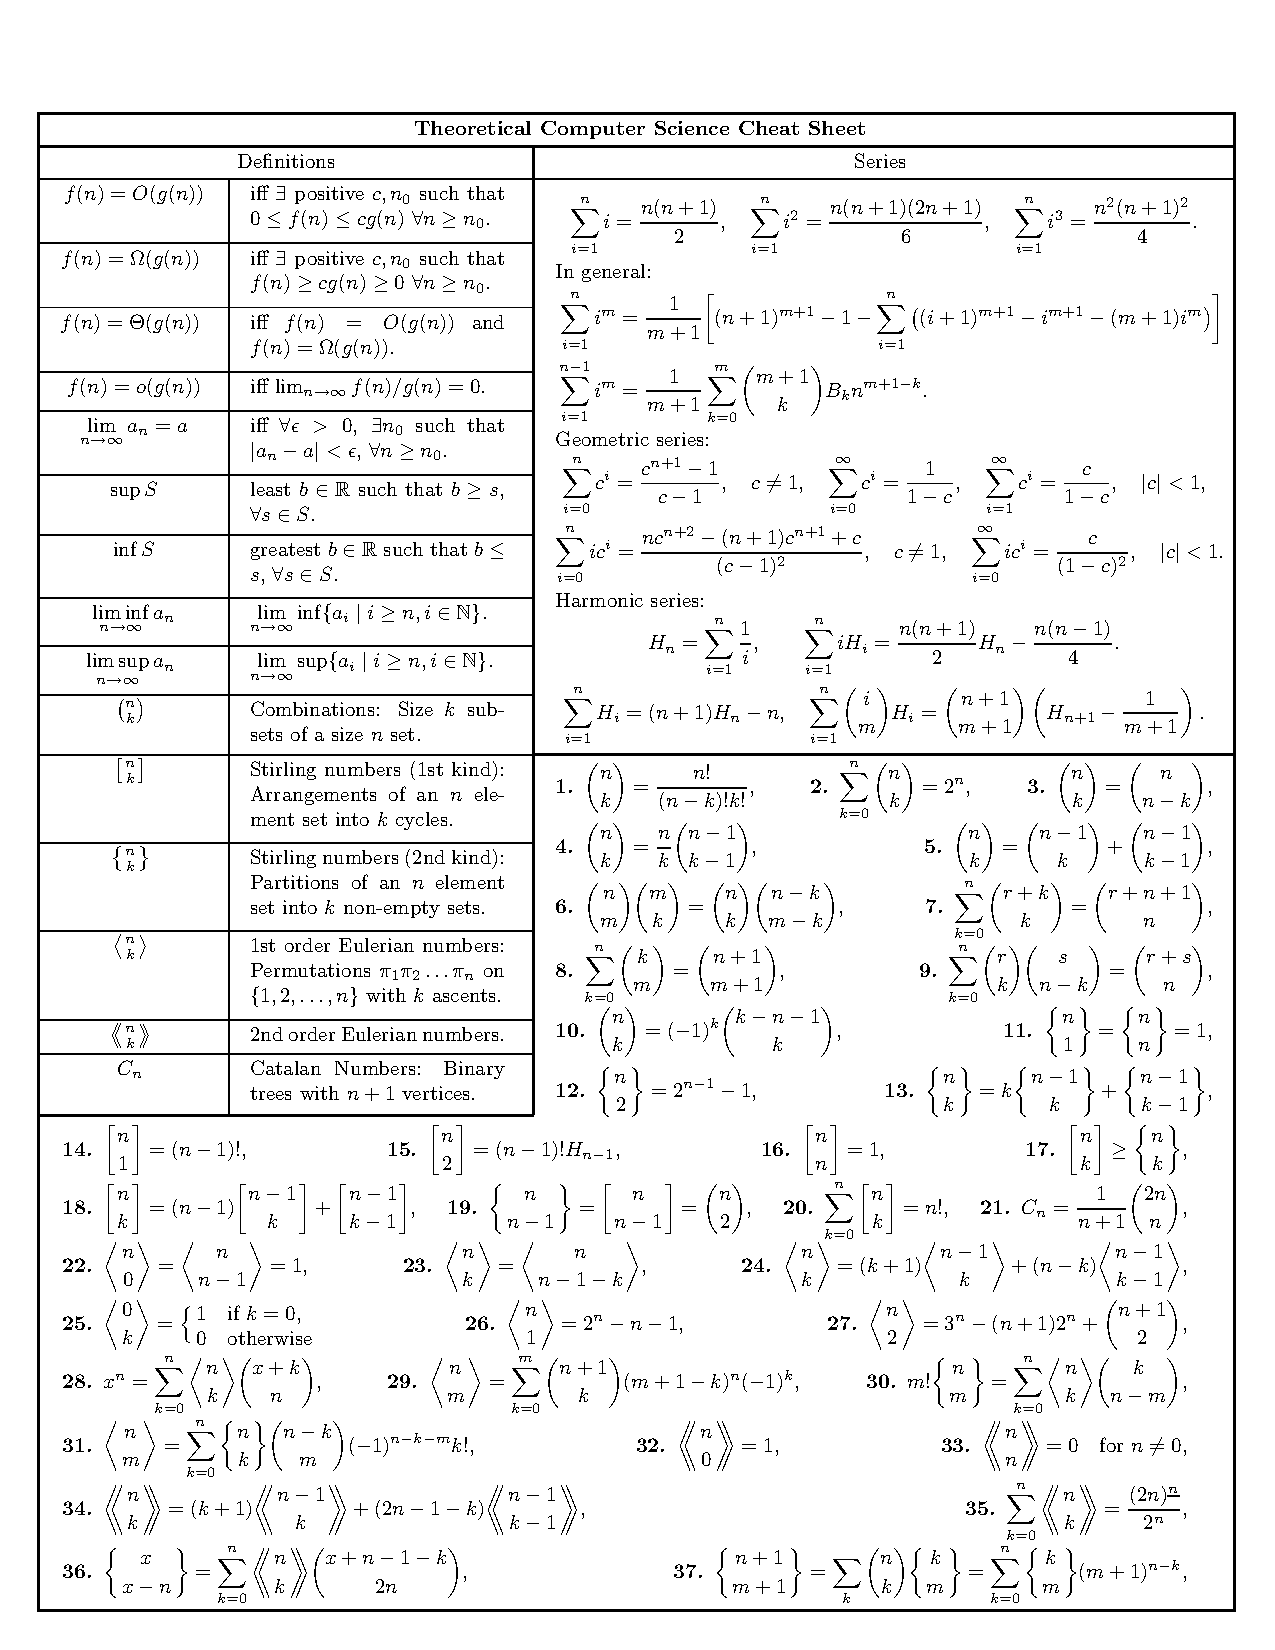
\includepdf[pages = 1-10]{pdf/cheat-sheet.pdf}
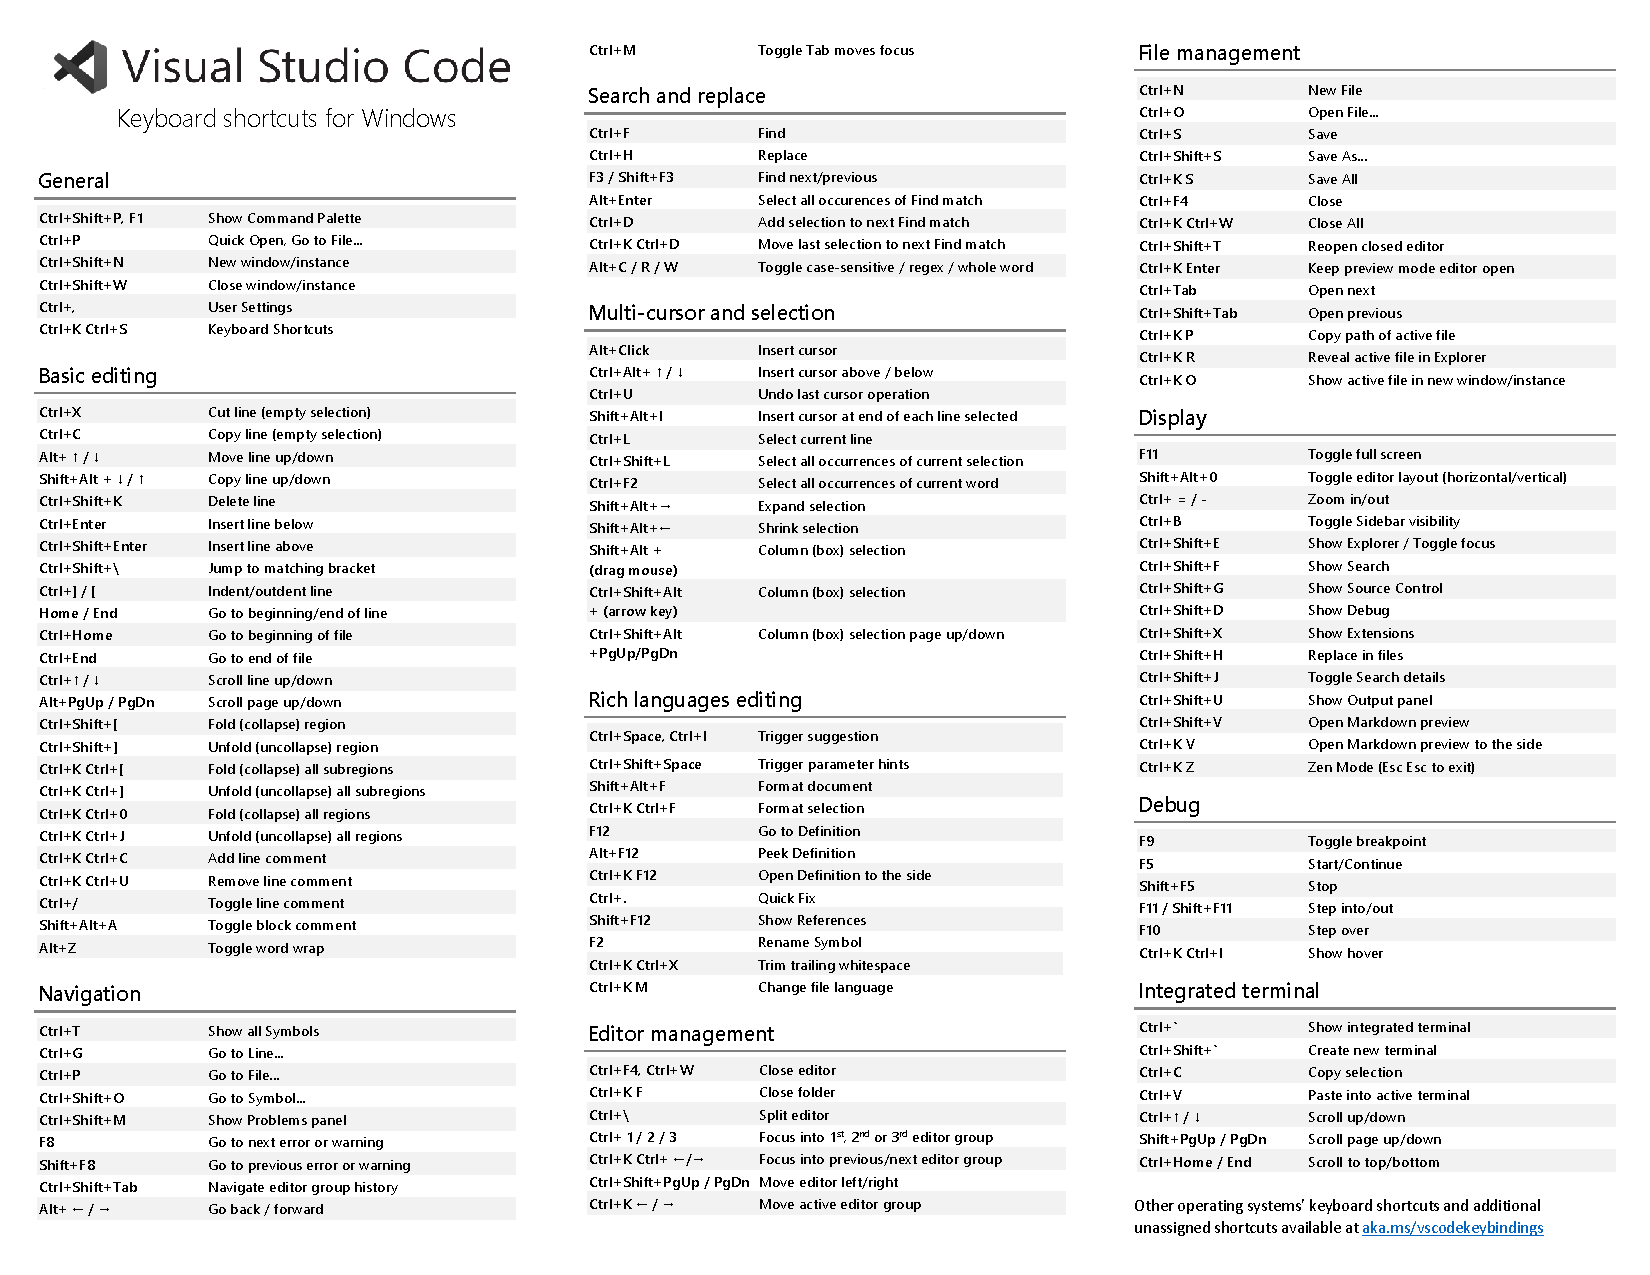
\includepdf[angle=90]{pdf/keyboard-shortcuts-windows.pdf}
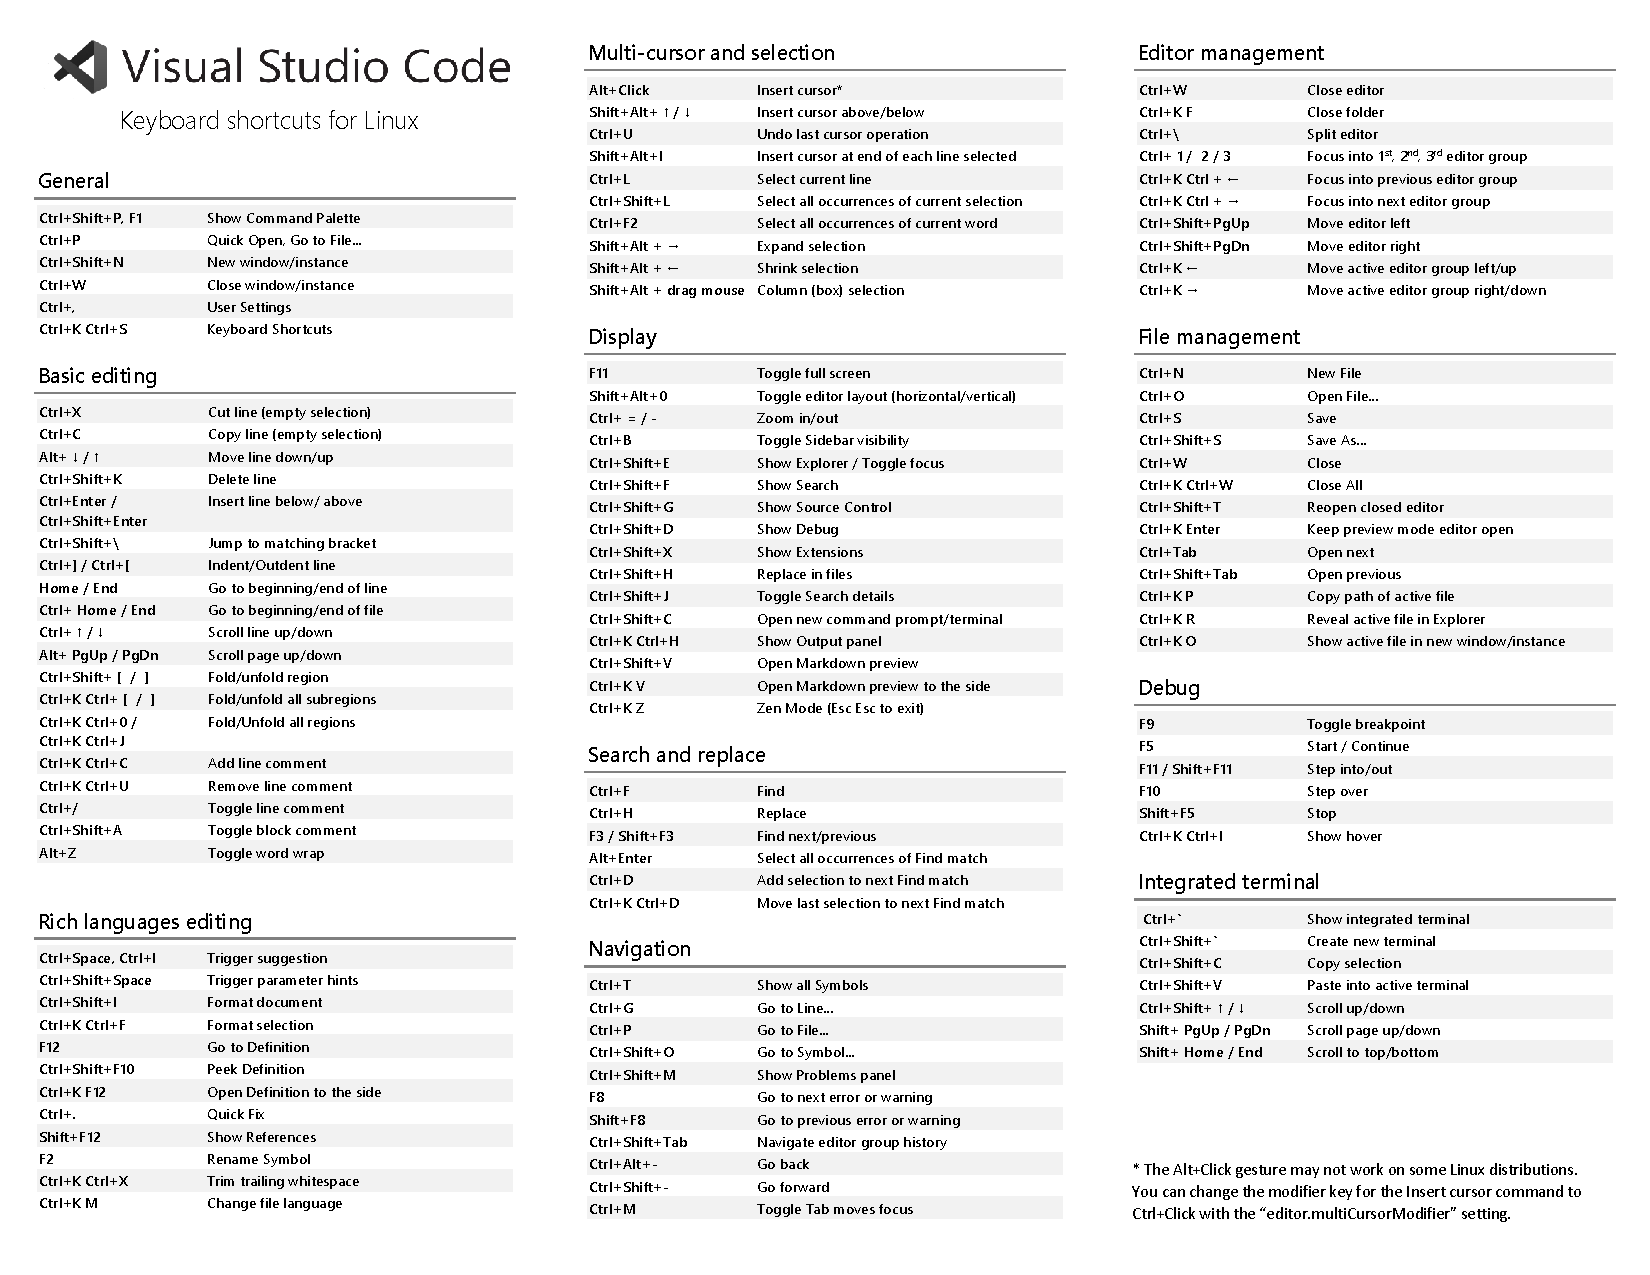
\includepdf[angle=270]{pdf/keyboard-shortcuts-linux.pdf}

\end{document}